\documentclass{article}[18pt]
\ProvidesPackage{format}
%Page setup
\usepackage[utf8]{inputenc}
\usepackage[margin=0.7in]{geometry}
\usepackage{parselines} 
\usepackage[english]{babel}
\usepackage{fancyhdr}
\usepackage{titlesec}
\hyphenpenalty=10000

\pagestyle{fancy}
\fancyhf{}
\rhead{Sam Robbins}
\rfoot{Page \thepage}

%Characters
\usepackage{amsmath}
\usepackage{amssymb}
\usepackage{gensymb}
\newcommand{\R}{\mathbb{R}}

%Diagrams
\usepackage{pgfplots}
\usepackage{graphicx}
\usepackage{tabularx}
\usepackage{relsize}
\pgfplotsset{width=10cm,compat=1.9}
\usepackage{float}

%Length Setting
\titlespacing\section{0pt}{14pt plus 4pt minus 2pt}{0pt plus 2pt minus 2pt}
\newlength\tindent
\setlength{\tindent}{\parindent}
\setlength{\parindent}{0pt}
\renewcommand{\indent}{\hspace*{\tindent}}

%Programming Font
\usepackage{courier}
\usepackage{listings}
\usepackage{pxfonts}

%Lists
\usepackage{enumerate}
\usepackage{enumitem}

% Networks Macro
\usepackage{tikz}


% Commands for files converted using pandoc
\providecommand{\tightlist}{%
	\setlength{\itemsep}{0pt}\setlength{\parskip}{0pt}}
\usepackage{hyperref}

% Get nice commands for floor and ceil
\usepackage{mathtools}
\DeclarePairedDelimiter{\ceil}{\lceil}{\rceil}
\DeclarePairedDelimiter{\floor}{\lfloor}{\rfloor}

% Allow itemize to go up to 20 levels deep (just change the number if you need more you madman)
\usepackage{enumitem}
\setlistdepth{20}
\renewlist{itemize}{itemize}{20}

% initially, use dots for all levels
\setlist[itemize]{label=$\cdot$}

% customize the first 3 levels
\setlist[itemize,1]{label=\textbullet}
\setlist[itemize,2]{label=--}
\setlist[itemize,3]{label=*}

% Definition and Important Stuff
% Important stuff
\usepackage[framemethod=TikZ]{mdframed}

\newcounter{theo}[section]\setcounter{theo}{0}
\renewcommand{\thetheo}{\arabic{section}.\arabic{theo}}
\newenvironment{important}[1][]{%
	\refstepcounter{theo}%
	\ifstrempty{#1}%
	{\mdfsetup{%
			frametitle={%
				\tikz[baseline=(current bounding box.east),outer sep=0pt]
				\node[anchor=east,rectangle,fill=red!50]
				{\strut Important};}}
	}%
	{\mdfsetup{%
			frametitle={%
				\tikz[baseline=(current bounding box.east),outer sep=0pt]
				\node[anchor=east,rectangle,fill=red!50]
				{\strut Important:~#1};}}%
	}%
	\mdfsetup{innertopmargin=10pt,linecolor=red!50,%
		linewidth=2pt,topline=true,%
		frametitleaboveskip=\dimexpr-\ht\strutbox\relax
	}
	\begin{mdframed}[]\relax%
		\centering
		}{\end{mdframed}}



\newcounter{lem}[section]\setcounter{lem}{0}
\renewcommand{\thelem}{\arabic{section}.\arabic{lem}}
\newenvironment{defin}[1][]{%
	\refstepcounter{lem}%
	\ifstrempty{#1}%
	{\mdfsetup{%
			frametitle={%
				\tikz[baseline=(current bounding box.east),outer sep=0pt]
				\node[anchor=east,rectangle,fill=blue!20]
				{\strut Definition};}}
	}%
	{\mdfsetup{%
			frametitle={%
				\tikz[baseline=(current bounding box.east),outer sep=0pt]
				\node[anchor=east,rectangle,fill=blue!20]
				{\strut Definition:~#1};}}%
	}%
	\mdfsetup{innertopmargin=10pt,linecolor=blue!20,%
		linewidth=2pt,topline=true,%
		frametitleaboveskip=\dimexpr-\ht\strutbox\relax
	}
	\begin{mdframed}[]\relax%
		\centering
		}{\end{mdframed}}
\lhead{Software Engineering}


\begin{document}
\begin{center}
\underline{\huge Scheduling and Risks II}
\end{center}
\section{Scheduling}
\subsection{Tracking Progress}
\begin{itemize}
	\item Do we understand customer's needs?
	\item Can we design a system to solve customer's problems or satisfy customer's needs?
	\item How long will it take to develop the system?
	\item How much will it cost to develop the system
\end{itemize}
\subsection{Project Scheduling}
\begin{enumerate}
	\item Capturing and Sequencing Activities
	\item Assigning resources and establishing durations
	\item Verifying the schedule and critical path
	\item Conducting a schedule risk analysis
	\item Updating the schedule
	\item Maintaining a baseline schedule
\end{enumerate}
\begin{itemize}
	\item Understand how to plan, monitor and control projects using PERT/CPM
	\begin{itemize}
		\item Program Evaluation and Review Technique
		\begin{itemize}
			\item A graphic representation of a project's schedule
			\item Shows the sequence of tasks
			\item Shows which tasks can be performed simultaneously
			\item Pert applies a 3-point weighted average duration estimate
$$T_e=(T_o+4\times T_m + T_p)\div 6$$
$T_e$ = Expected Duration\\
$T_o$ = Optimistic Duration\\
$T_m$ = Most Likely Duration\\
$T_p$ = Pessimistic Duration
		\end{itemize}
	
		\item Critical path method
		\begin{itemize}
			\item Analysis of path among milestones
			\item Identify minimum amount of time to complete the project
			\item Reveals those activities that are most critical to completing the project on time
			\item Calculate available time, real time and slack time as well as latest and earliest start time
		\end{itemize}
	\end{itemize}
	\item Determine the earliest finish, the latest start, the latest finish and slack times for each activity
	\item Understand the impact of variability in activity times on the project completion time
\end{itemize}
\subsection{Schedule Risks}
A schedule is one of the project drivers that is most susceptible to risk
\begin{itemize}
	\item Schedules comprise multiple inter-dependant activities, each of which usually contain multiple uncertainties
	\item \textit{Proactive scheduling}: Add time up front to deal with uncertainties
	\item \textit{Reactive scheduling}: Incorporate a process to react to and absorb disruptions
	\item Mainly affects the critical path - other disruptions can often be easily absorbed
	\item Therefore it is important that the critical path is protected
\end{itemize} 
\section{Risks}
A risk can be measured by its likelihood $\times$ the impact 
\begin{center}
	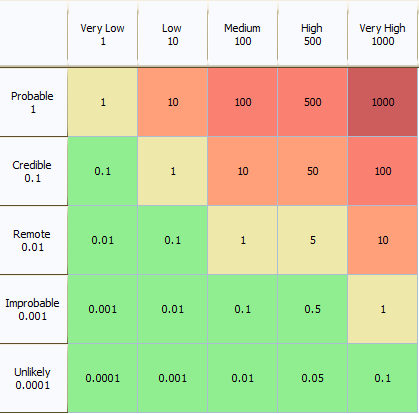
\includegraphics[scale=0.5]{risk}
\end{center}
A risk is an unwanted event that has negative consequences. Project managers must engage in risk management to understand and control the risks on their project\\
\\
Distinguish risks from other project events by looking for:
\begin{enumerate}
	\item Loss associated with the event - risk impact
	\item Likelihood the event will happen - risk probability
	\item Degree to which we can change the outcome - risk control
\end{enumerate}
There are two major sources of risk
\begin{itemize}
	\item Generic risk
	\item Project risk
\end{itemize}
\subsection{Risk management}
Risk management is concerned with identifying risks and drawing up plans to minimise their effect on a project\\
\\
A risk is a probability that some adverse circumstance will occur, they can be typed:
\begin{itemize}
	\item Project risks affect schedule or resources
	\item Product risks affect the quality or performance of the software being developed
	\item Business risks affect the organisation developing or procuring the software
\end{itemize}
\begin{center}
	\includegraphics[scale=0.5]{"risk management"}
\end{center}
\subsection{Risk identification}
May be team activities or based on the individual project manager's experience\\
A checklist of common risks may be used to identify risks in a project
\begin{itemize}
	\item Technology risks
	\item People risks
	\item Organisational risks
	\item Tools risk
	\item Requirements risks
	\item Estimation risks
\end{itemize}
\subsection{Risk analysis}
\begin{itemize}
	\item Asses probability and seriousness of each risk
	\item Probability may be very low, low, moderate, high or very high
	\item Risk consequences might be catastrophic, serious, tolerable or insignificant
\end{itemize}
\subsection{Risk mitigation}
Consider each risk and develop a strategy to manage that risk:
\begin{itemize}
	\item Avoidance strategies - the probability that the risk will arise is reduced
	\item Minimisation strategies - the impact of the risk on the project or product will be reduced
	\item Contingency plans - if the risk arises, contingency plans are plans to deal with that risk
\end{itemize}
\subsection{Risk monitoring}
Assess each identified risks regularly to decide whether it is becoming less or more probable\\
\\
Risk monitoring tracks progress
\begin{itemize}
	\item Assess whether a predicted risk occurs
	\item Assess whether the effects of the risk have changed
	\item Ensures that risk aversion steps are defined and properly applied
	\item Collects information that can be used in the future
\end{itemize}
Each key risk should be discussed at management progress meetings\\
When problems occur we need to be able to identify why

\end{document}